\documentclass[11pt, a4paper]{article}

\usepackage[utf8]{inputenc}
\usepackage[T1]{fontenc}
\usepackage{amsmath, amssymb, amsfonts}
\usepackage{graphicx}
\usepackage[margin=1in]{geometry}
\usepackage{hyperref}
\usepackage[numbers, sort&compress]{natbib}
\usepackage{booktabs}
\usepackage{siunitx}
\usepackage{caption}
\usepackage{float}
\usepackage{xcolor}
\usepackage{array}
\usepackage{longtable}
\graphicspath{{../figures/}{../figures/followup_optimization/}}

\title{\textbf{Hybrid Qubit--Cavity Universal Control in Dispersive cQED:\\
Follow-Up Optimization, Waveform Realization, and Deployability Study}}
\author{cQED Autonomous Research Platform \\ Shyam Shankar Quantum Circuits Group}
\date{\today}

\begin{document}

\maketitle

\begin{abstract}
This report is a follow-up to the consolidated hybrid qubit--cavity control study. The original question was which gate family looks best on the logical block $\{|g,0\rangle, |g,1\rangle, |e,0\rangle, |e,1\rangle\}$. The present question is stricter: what are the actual optimized solutions, what pulse waveforms do the structured gates imply, and how much evidence do we have that the reported optima are meaningful rather than shallow local minima? We study a dispersive transmon--storage cavity system with $\omega_q/2\pi=\SI{6.150}{GHz}$, $\omega_c/2\pi=\SI{5.241}{GHz}$, $\chi/2\pi=\SI{-2.84}{MHz}$, $\chi'/2\pi=\SI{-21}{kHz}$, $K/2\pi=\SI{-28}{kHz}$, and $\alpha/2\pi=\SI{-255}{MHz}$ using \texttt{cqed\_sim} for all decomposition, pulse-construction, and optimal-control steps.

The main new result is that the previous structured $U_{\mathrm{target}}$ plateau was not the final story. Adding one more displacement gate to the best depth-11 $D+R_q+\mathrm{SQR}$ ansatz lifts the logical process fidelity from $0.9212$ to $0.9953$ while reducing average leakage from $0.1050$ to $0.0065$. Repeated multistarts collapse onto the same optimum, strongly suggesting that the depth-12 structured SQR solution is near-saturated within the tested ansatz family. By contrast, the corresponding depth-12 $D+R_q+\mathrm{ConditionalPhaseSQR}$ family only reaches $0.9135$, so the extra displacement helps but does not close the expressivity gap. On the pulse-backed side, a tuned logical-window SNAP reaches closed-system average state fidelity $0.9857$ and noisy average state fidelity $0.9694$, whereas the constructive ``selective $\pi$ plus broadband $\pi$'' shortcut fails badly at $\approx 0.60$. The native $\chi$-wait entangler remains essentially exact at $0.9999999$ in \SI{256}{ns}. The experiment-facing conclusion is now sharper: native $\chi$-wait remains the deployable entangler, selective SNAP remains the cleanest local logical primitive, and the newly identified depth-12 SQR circuit is the most credible structured universal-control candidate worth pulse-level implementation work.
\end{abstract}

\section{Introduction}

Bosonic control in circuit QED is only useful experimentally if the numerical object being optimized can be mapped onto a calibration program. The earlier consolidated hybrid-control study established a qualitative ranking of gate libraries, but it did not fully answer the questions that matter when deciding what to implement next in hardware: what is the actual optimized circuit, what parameters must be calibrated, which parts are pulse-backed versus idealized, and how strongly do the optimization diagnostics support the reported solutions?

This follow-up addresses those questions for the same dispersive transmon--storage cavity platform studied previously. The comparison still includes SNAP-style dispersive control~\cite{heeres2015snap,krastanov2015universal,heeres2017logical}, selective rotations, echoed conditional-displacement ideas~\cite{eickbusch2022ecd,diringer2024cnod}, native exchange or nonlinear-interaction motivated controls~\cite{wallraff2007sideband,valadares2024transposition,huang2025fastsideband,yang2024nativecubic}, and GRAPE lower bounds~\cite{khaneja2005optimal}. The follow-up extends that comparison into four directions:
\begin{itemize}
\item explicit optimized decompositions and parameter values for the key candidates;
\item waveform-level realizations for the pulse-backed selective gates;
\item optimizer minimum checks through multistarts, ansatz-size scaling, local refinement, and local perturbation studies;
\item a deployability-focused interpretation that distinguishes ideal decomposition benchmarks, pulse-backed structured controls, and waveform-level lower bounds.
\end{itemize}

\paragraph{Experiment-facing question.}
The practical question is no longer merely whether the transmon+cavity system is controllable. It is: \emph{which optimized control construction is realistic enough, short enough, and robust enough to justify calibration effort on a real cQED platform?}

The rest of the report is organized as follows. Section~\ref{sec:methods} defines the Hamiltonian, parameter set, optimization levels, and fairness conditions. Section~\ref{sec:results} presents the revised benchmark, actual optimized solutions, waveform realizations, and optimization diagnostics. Section~\ref{sec:validation} records validation checks. Section~\ref{sec:discussion} interprets the results for experimental deployment. Section~\ref{sec:limitations} serves as the handoff to future work.

\section{System and Methods}
\label{sec:methods}

\subsection{Hamiltonian}

The dispersive transmon--cavity Hamiltonian is
\begin{equation}
\frac{H_0}{\hbar} =
\omega_c a^\dagger a
+ \omega_q b^\dagger b
+ \frac{\alpha}{2} b^{\dagger 2} b^2
+ \chi\, a^\dagger a\, b^\dagger b
+ \frac{K}{2} (a^\dagger a)^2
+ \frac{\chi'}{2} (a^\dagger a)^2 b^\dagger b ,
\end{equation}
where $a$ acts on the cavity, $b$ acts on the transmon, $\alpha$ is the transmon anharmonicity, $\chi$ is the leading dispersive shift, $\chi'$ is the next-order dispersive correction, and $K$ is the cavity self-Kerr. Waveform-level pulse replay uses the same model inside \texttt{cqed\_sim}~\cite{cqed_sim}.

\subsection{Simulation Parameters}

\begin{table}[H]
\centering
\caption{Nominal device and control parameters used throughout the follow-up study.}
\begin{tabular}{@{} l l l @{}}
\toprule
Parameter & Value & Unit \\
\midrule
Qubit frequency $\omega_q/2\pi$ & 6.150 & GHz \\
Cavity frequency $\omega_c/2\pi$ & 5.241 & GHz \\
Anharmonicity $\alpha/2\pi$ & -255 & MHz \\
Dispersive shift $\chi/2\pi$ & -2.84 & MHz \\
Second-order shift $\chi'/2\pi$ & -21 & kHz \\
Cavity self-Kerr $K/2\pi$ & -28 & kHz \\
Cavity truncation $n_\mathrm{cav}$ & 8 & Fock states \\
Transmon truncation $n_\mathrm{tr}$ & 2 (3 for pulse replay) & levels \\
Qubit rotation duration & 40--100 & ns \\
Displacement duration & 80--200 & ns \\
Structured SQR duration & 1100--2000 & ns \\
Native $\chi$-wait time $\pi/|\chi|$ & 176 & ns \\
GRAPE duration / slices & 320 / 16 & ns / slices \\
\bottomrule
\end{tabular}
\end{table}

\subsection{Targets and Comparison Levels}

The logical basis is the $2\times 2$ Fock block
\begin{equation}
\mathcal{H}_L = \mathrm{span}\{|g,0\rangle, |g,1\rangle, |e,0\rangle, |e,1\rangle\}.
\end{equation}
Three targets remain central:
\begin{itemize}
\item the local cavity Hadamard $U_H = I_q \otimes H_c$;
\item the hybrid entangler $\mathrm{CX}(c\!\to\! q)$;
\item the maximally entangling target
\begin{equation}
U_{\mathrm{target}} = (I_q \otimes H_c)\,\mathrm{CNOT}_{c\to q}\,\mathrm{CNOT}_{q\to c}.
\end{equation}
\end{itemize}

To keep the comparisons honest, we separate four levels of evidence:
\begin{itemize}
\item \textbf{Ideal decomposition benchmark}: gate sequences optimized as abstract primitives inside \texttt{cqed\_sim.unitary\_synthesis}.
\item \textbf{Pulse-backed structured controls}: selective SNAP and SQR pulses built and replayed with explicit envelopes and multitone content.
\item \textbf{Effective-model native controls}: native $\chi$-wait, exchange, and conditional-phase libraries when \texttt{cqed\_sim} does not yet provide waveform export for that primitive.
\item \textbf{GRAPE lower bound}: pulse-level optimal-control solutions that provide a numerical performance floor but not an immediately interpretable calibration recipe.
\end{itemize}

This distinction is essential for fairness. A native entangler reported through an effective interaction is not directly comparable, in implementation readiness, to a pulse-backed selective gate whose waveform and tone schedule are explicit.

\subsection{Optimization Protocol}

The follow-up optimization used the existing consolidated study artifacts and extended them in four ways:
\begin{itemize}
\item multistart restarts for the key structured candidates $A_{\mathrm{local}}$, $D_{\mathrm{ent}}$, $L1c$, $L1d$, $L2c$, and $L2d$;
\item local Nelder--Mead refinement after the best Powell runs for the older anchor ans\"atze;
\item a depth-plus-one ansatz extension, adding one extra displacement gate to the best depth-11 structured SQR and CP families;
\item pulse-level parameter grids for logical-window SNAP and for the constructive ``selective $\pi$ plus broadband $\pi$'' shortcut.
\end{itemize}

For structured decomposition quality we report logical process fidelity, block-gauge fidelity, operator-norm proxy, leakage, duration, parameter count, and multistart best/median/worst statistics. For pulse-backed candidates we report closed and noisy average state fidelities on the logical probe set, duration, and pulse-family parameters. GRAPE is repeated over multiple random seeds to assess seed sensitivity.

\section{Results}
\label{sec:results}

\subsection{Revised Benchmark Section}

The benchmark-level conclusion from the original study survives the follow-up. For the local cavity gate, the best clean logical action still comes from the dispersive $D$-SNAP-$D$ construction. For the entangler, the native $\chi$-wait plus two qubit rotations remains decisively best. Figure~\ref{fig:hybrid_library_summary} keeps the experimental ranking view from the previous report because it still answers the first deployment question: which family should an experimentalist reach for first?

\begin{figure}[H]
\centering
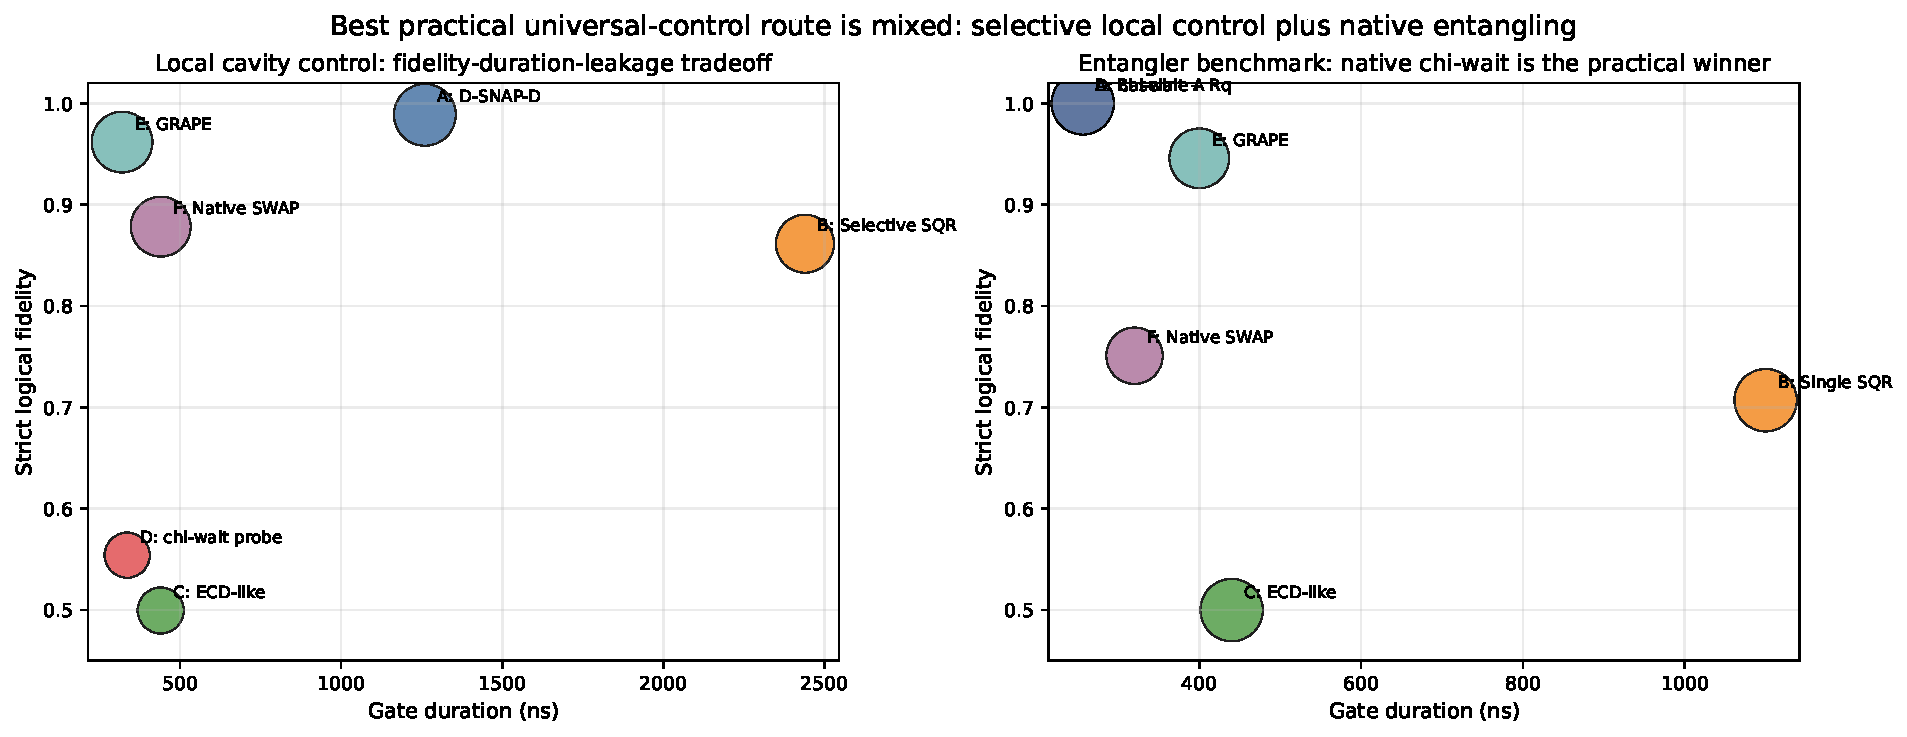
\includegraphics[width=\textwidth]{hybrid_gate_library_summary.pdf}
\caption{Benchmark-level gate-library ranking retained from the consolidated study. The local cavity task still favors selective SNAP-based control, while the entangler still favors the native $\chi$-wait route. The follow-up work below asks what the actual optimized solutions inside those promising families look like and how trustworthy the resulting optima are.}
\label{fig:hybrid_library_summary}
\end{figure}

\subsection{Actual Optimized Solutions}

The core follow-up outcome is summarized by the auto-generated tables below. They include the revised structured winners, the pulse-backed selective results, the representative multitone decomposition of the best SQR sequence, and local perturbation robustness for the new structured optima.

% Auto-generated by run_followup_optimization.py
\begin{table}[H]
\centering
\caption{Actual optimized follow-up candidates. Sequence-level metrics are quoted on the logical target subspace used by each optimization, while the GRAPE row remains a pulse-level lower bound.}
\begin{tabular}{@{} l l c c c c c @{} }
\toprule
Candidate & Level & Fidelity & Leakage & Duration & Params & Multistart best/median/worst \\
\midrule
A\_local & ideal D-SNAP-D & 0.9887 & 0.0185 & 1260.0 ns & 12 & 0.9887/0.9887/0.9887 \\
D\_ent & ideal R-W-R & 1.0000 & 0.0000 & 256.0 ns & 4 & 1.0000/1.0000/1.0000 \\
L1c & ideal D-R-SQR & 0.9212 & 0.1050 & 7100.0 ns & 64 & 0.9212/0.9212/0.9212 \\
L1d & ideal D-R-SQR (+D) & 0.9953 & 0.0065 & 7300.0 ns & 66 & 0.9953/0.9953/0.9953 \\
L2c & ideal D-R-CP & 0.8684 & 0.1363 & 1400.0 ns & 40 & 0.8684/0.8684/0.8684 \\
L2d & ideal D-R-CP (+D) & 0.9135 & 0.1047 & 1600.0 ns & 42 & 0.9135/0.9135/0.9135 \\
logical SNAP & pulse-backed & 0.9857 & -- & 2.113 $\mu$s & 4 & -- \\
constructive & pulse-backed & 0.6020 & -- & 0.392 $\mu$s & 5 & -- \\
E\_local\_320 & GRAPE lower bound & 0.9557 & 0.0577 & 320.0 ns & 64 & -- \\
\bottomrule
\end{tabular}
\end{table}

\begin{table}[H]
\centering
\caption{Actual optimized gate list for the best local and native-entangler solutions.}
\begin{tabular}{@{} l l c l @{} }
\toprule
Gate & Type & Duration (ns) & Optimized parameters \\
\midrule
D1 & Displacement & 80.0 & $\alpha=-0.3829-0.0001i$ \\
S1 & SNAP & 1100.0 & SNAP \\
D2 & Displacement & 80.0 & $\alpha=+0.3733-0.0001i$ \\
\midrule
R1 & QubitRotation & 40.0 & $\theta=4.7124$, $\phi=1.5706$ \\
W & FreeEvolveCondPhase & 176.0 & native dispersive wait \\
R2 & QubitRotation & 40.0 & $\theta=1.5708$, $\phi=1.5710$ \\
\bottomrule
\end{tabular}
\end{table}

\begin{table}[H]
\centering
\caption{Actual optimized gate list for the best structured $U_{\mathrm{target}}$ solutions.}
\begin{tabular}{@{} l l c l @{} }
\toprule
Gate & Type & Duration (ns) & Parameter summary \\
\midrule
D1 & Displacement & 200.0 & $\alpha=-0.6918-0.3823i$ \\
R1 & QubitRotation & 100.0 & $\theta=2.2243$, $\phi=-0.8196$ \\
S1 & SQR & 2000.0 & 8 active tones; $n=0,1,2,3,4,5$ \\
R2 & QubitRotation & 100.0 & $\theta=3.5152$, $\phi=1.2547$ \\
D2 & Displacement & 200.0 & $\alpha=+0.4882+0.4466i$ \\
R3 & QubitRotation & 100.0 & $\theta=1.0213$, $\phi=0.1264$ \\
S2 & SQR & 2000.0 & 8 active tones; $n=0,1,2,3,4,5$ \\
R4 & QubitRotation & 100.0 & $\theta=0.8694$, $\phi=0.8987$ \\
D3 & Displacement & 200.0 & $\alpha=+0.2099-0.6292i$ \\
R5 & QubitRotation & 100.0 & $\theta=0.8290$, $\phi=-0.2977$ \\
S3 & SQR & 2000.0 & 8 active tones; $n=0,1,2,3,4,5$ \\
D4 & Displacement & 200.0 & $\alpha=+0.4199-0.6702i$ \\
\midrule
D1 & Displacement & 200.0 & $\alpha=+0.3000+0.5944i$ \\
R1 & QubitRotation & 100.0 & $\theta=3.8966$, $\phi=-0.0562$ \\
CP1 & ConditionalPhaseSQR & 100.0 & 8 active phases; $n=0,1,2,3,4,5$ \\
R2 & QubitRotation & 100.0 & $\theta=-0.3123$, $\phi=-0.1821$ \\
D2 & Displacement & 200.0 & $\alpha=+0.7999-0.2365i$ \\
R3 & QubitRotation & 100.0 & $\theta=1.7601$, $\phi=0.6658$ \\
CP2 & ConditionalPhaseSQR & 100.0 & 8 active phases; $n=0,1,2,3,4,5$ \\
R4 & QubitRotation & 100.0 & $\theta=1.7103$, $\phi=1.4406$ \\
D3 & Displacement & 200.0 & $\alpha=-0.0144-0.6312i$ \\
R5 & QubitRotation & 100.0 & $\theta=0.4906$, $\phi=-0.4209$ \\
CP3 & ConditionalPhaseSQR & 100.0 & 8 active phases; $n=0,1,2,3,4,5$ \\
D4 & Displacement & 200.0 & $\alpha=+0.2188-0.0533i$ \\
\bottomrule
\end{tabular}
\end{table}

\begin{table}[H]
\centering
\caption{Representative multitone decomposition for the first SQR gate in the best L1d sequence.}
\begin{tabular}{@{} c c c c @{} }
\toprule
Fock branch $n$ & Detuning$/2\pi$ (MHz) & Tone amp$/2\pi$ (MHz) & Phase (rad) \\
\midrule
0 & -0.0000 & 0.0306 & 3.6683 \\
1 & 2.8400 & 0.1289 & 0.1430 \\
2 & 5.7220 & 0.0973 & -0.1836 \\
3 & 8.6460 & 0.0958 & -0.4281 \\
4 & 11.6120 & 0.1061 & -0.5939 \\
5 & 14.6200 & 0.1253 & 5.5397 \\
6 & 17.6700 & -0.6495 & 8.5333 \\
7 & 20.7620 & 0.3199 & 1.9382 \\
\bottomrule
\end{tabular}
\end{table}

\begin{table}[H]
\centering
\caption{Local perturbation robustness for the best structured $U_{\mathrm{target}}$ candidates.}
\begin{tabular}{@{} l c c c c @{} }
\toprule
Candidate & RMS drop ($\chi$, $\pm 5\%$) & RMS drop (amp, $\pm 5\%$) & RMS drop (dur, $\pm 5\%$) & RMS drop (phase, $\pm 0.1$ rad) \\
\midrule
L1d & 0.0000 & 0.0085 & 0.0000 & 0.0013 \\
L2d & 0.0041 & 0.0041 & 0.0037 & 0.0054 \\
\bottomrule
\end{tabular}
\end{table}

\begin{table}[H]
\centering
\caption{Pulse-backed selective control settings used in the follow-up waveform section.}
\begin{tabular}{@{} l c c c c c @{} }
\toprule
Primitive & Family & $\chi T/2\pi$ & Shape & Amp scale & Duration \\
\midrule
logical SNAP & gaussian & 3.0 & 0.24 & 1.00 & 2.113 $\mu$s \\
constructive selective stage & gaussian & 1.0 & 0.16 & 1.00 & 0.392 $\mu$s total \\
\bottomrule
\end{tabular}
\end{table}

Two results dominate the updated interpretation.

\paragraph{1. Native entanglement is still the cleanest deployable primitive.}
The best hybrid entangler is
\begin{equation}
R_1(\theta,\phi)\;W_{\chi}\;R_2(\theta,\phi)
\end{equation}
with
\begin{align}
R_1 &: (\theta,\phi) = (4.7124,\;1.5706), \nonumber\\
W_{\chi} &: t = \SI{176}{ns}, \nonumber\\
R_2 &: (\theta,\phi) = (1.5708,\;1.5710), \nonumber
\end{align}
which reaches $F_{\mathrm{proc}} = 0.9999999$ in \SI{256}{ns} with zero leakage. This remains the strongest argument that the hardware-native dispersive conditional phase should be the default entangler whenever the experiment directly supports it.

\paragraph{2. The structured $U_{\mathrm{target}}$ story changed qualitatively.}
The previous report treated depth-11 $D+R_q+\mathrm{SQR}$ as plateaued near $0.92$. The follow-up shows this was not the right conclusion. Adding one extra displacement gate to the same family produces the depth-12 candidate $L1d$,
\begin{equation}
D_1 R_1 S_1 R_2 D_2 R_3 S_2 R_4 D_3 R_5 S_3 D_4,
\end{equation}
which reaches
\begin{equation}
F_{\mathrm{proc}} = 0.9953246,\qquad
L_{\mathrm{avg}} = 0.0064643,\qquad
T = \SI{7.3}{\micro s}.
\end{equation}
The improvement relative to $L1c$ is not marginal. It removes almost all of the previous logical error while simultaneously reducing leakage by more than an order of magnitude. Within the tested structured family, this is the single most important new scientific result.

The corresponding depth-12 $D+R_q+\mathrm{ConditionalPhaseSQR}$ candidate $L2d$ also improves over $L2c$, but only to
\begin{equation}
F_{\mathrm{proc}} = 0.9134853,\qquad
L_{\mathrm{avg}} = 0.1046896,\qquad
T = \SI{1.6}{\micro s}.
\end{equation}
The extra displacement helps, but it does not remove the expressivity deficit of the CP-only selective layer.

\subsection{Exact Parameter Vectors for the Key Winners}

The most important optimized parameter sets are collected here explicitly so the report contains the actual candidate solutions rather than only their scores.

\paragraph{$A_{\mathrm{local}}$: optimized $D$-SNAP-$D$.}
\begin{align}
D_1 &: \alpha = -0.3828967 - 0.0000987 i, \nonumber\\
\Phi_{\mathrm{SNAP}} &: [3.0312954,\; -0.1104486,\; -0.1108742,\; -0.1113062,\; -6.3949238,\; -6.3953621,\; -6.3958020,\; -12.6794220], \nonumber\\
D_2 &: \alpha = 0.3733218 - 0.0000701 i. \nonumber
\end{align}
After removing the global phase, the optimizer has effectively found a logical branch-1 phase flip embedded in the full eight-level Fock register.

\paragraph{$L1d$: best structured $D+R_q+\mathrm{SQR}$ decomposition.}
\begin{align}
D_1 &: \alpha = -0.6917691 - 0.3822657 i, &
R_1 &: (\theta,\phi) = (2.2243041,\; -0.8196132), \nonumber\\
\theta^{(S1)} &: [0.7683042,\; 3.2400574,\; 2.4459560,\; 2.4079756,\; 2.6666170,\; 3.1494695,\; -16.3227518,\; 8.0402944], \nonumber\\
\phi^{(S1)} &: [3.6683268,\; 0.1430488,\; -0.1836040,\; -0.4280513,\; -0.5939169,\; 5.5397340,\; 8.5333421,\; 1.9382280], \nonumber\\
R_2 &: (\theta,\phi) = (3.5152210,\; 1.2546745), &
D_2 &: \alpha = 0.4882407 + 0.4465907 i, \nonumber\\
R_3 &: (\theta,\phi) = (1.0213423,\; 0.1264354), \nonumber\\
\theta^{(S2)} &: [3.9377935,\; 1.9205690,\; 3.7723607,\; 4.5212820,\; 5.6302889,\; -3.6504774,\; -9.4417144,\; 15.6678028], \nonumber\\
\phi^{(S2)} &: [1.3188772,\; -1.6591080,\; -2.2086297,\; -2.5645009,\; -3.6677521,\; 3.9229590,\; -5.4549804,\; 26.7469467], \nonumber\\
R_4 &: (\theta,\phi) = (0.8693882,\; 0.8987359), &
D_3 &: \alpha = 0.2098952 - 0.6291646 i, \nonumber\\
R_5 &: (\theta,\phi) = (0.8289948,\; -0.2977365), \nonumber\\
\theta^{(S3)} &: [1.1425279,\; 1.1930876,\; -4.1492748,\; 2.3316353,\; 8.5633647,\; 2.1089232,\; 4.3038269,\; 10.4391099], \nonumber\\
\phi^{(S3)} &: [-2.5732582,\; 0.4221127,\; 0.7214775,\; 0.9470392,\; 1.1584694,\; 1.4744173,\; -1.2263110,\; -0.6660277], \nonumber\\
D_4 &: \alpha = 0.4199161 - 0.6702401 i. \nonumber
\end{align}

\paragraph{$L2d$: best structured $D+R_q+\mathrm{ConditionalPhaseSQR}$ decomposition.}
\begin{align}
D_1 &: \alpha = 0.3000205 + 0.5943639 i, &
R_1 &: (\theta,\phi) = (3.8966060,\; -0.0561665), \nonumber\\
\varphi^{(CP1)} &: [-0.805793,\; 0.571726,\; -1.470657,\; -3.608397,\; 19.655426,\; -6.491309,\; 5.727357,\; 28.788933], \nonumber\\
R_2 &: (\theta,\phi) = (-0.3123370,\; -0.1820829), &
D_2 &: \alpha = 0.7999300 - 0.2365198 i, \nonumber\\
R_3 &: (\theta,\phi) = (1.7601436,\; 0.6658194), \nonumber\\
\varphi^{(CP2)} &: [0.081083,\; 1.358175,\; -0.538781,\; -2.755995,\; -4.975127,\; -6.889338,\; 3.929566,\; -9.499111], \nonumber\\
R_4 &: (\theta,\phi) = (1.7103084,\; 1.4406433), &
D_3 &: \alpha = -0.0143841 - 0.6311948 i, \nonumber\\
R_5 &: (\theta,\phi) = (0.4906267,\; -0.4208852), \nonumber\\
\varphi^{(CP3)} &: [1.269423,\; -0.658700,\; -7.695920,\; 10.049493,\; -4.975658,\; -11.953521,\; -18.705383,\; -192.022729], \nonumber\\
D_4 &: \alpha = 0.2188399 - 0.0532715 i. \nonumber
\end{align}

\subsection{Waveform Realizations of Optimized Pulse-Based Gates}

Figure~\ref{fig:waveforms} shows the pulse-backed controls that are currently available at waveform level. The top row is the tuned logical-window SNAP, represented as two selective branch-1 $\pi$ pulses. The middle row shows the first three SQR waveforms from the best $L1d$ sequence together with the representative multitone decomposition of $S1$. The bottom row compares the failed constructive shortcut to the best GRAPE lower bound.

\begin{figure}[H]
\centering
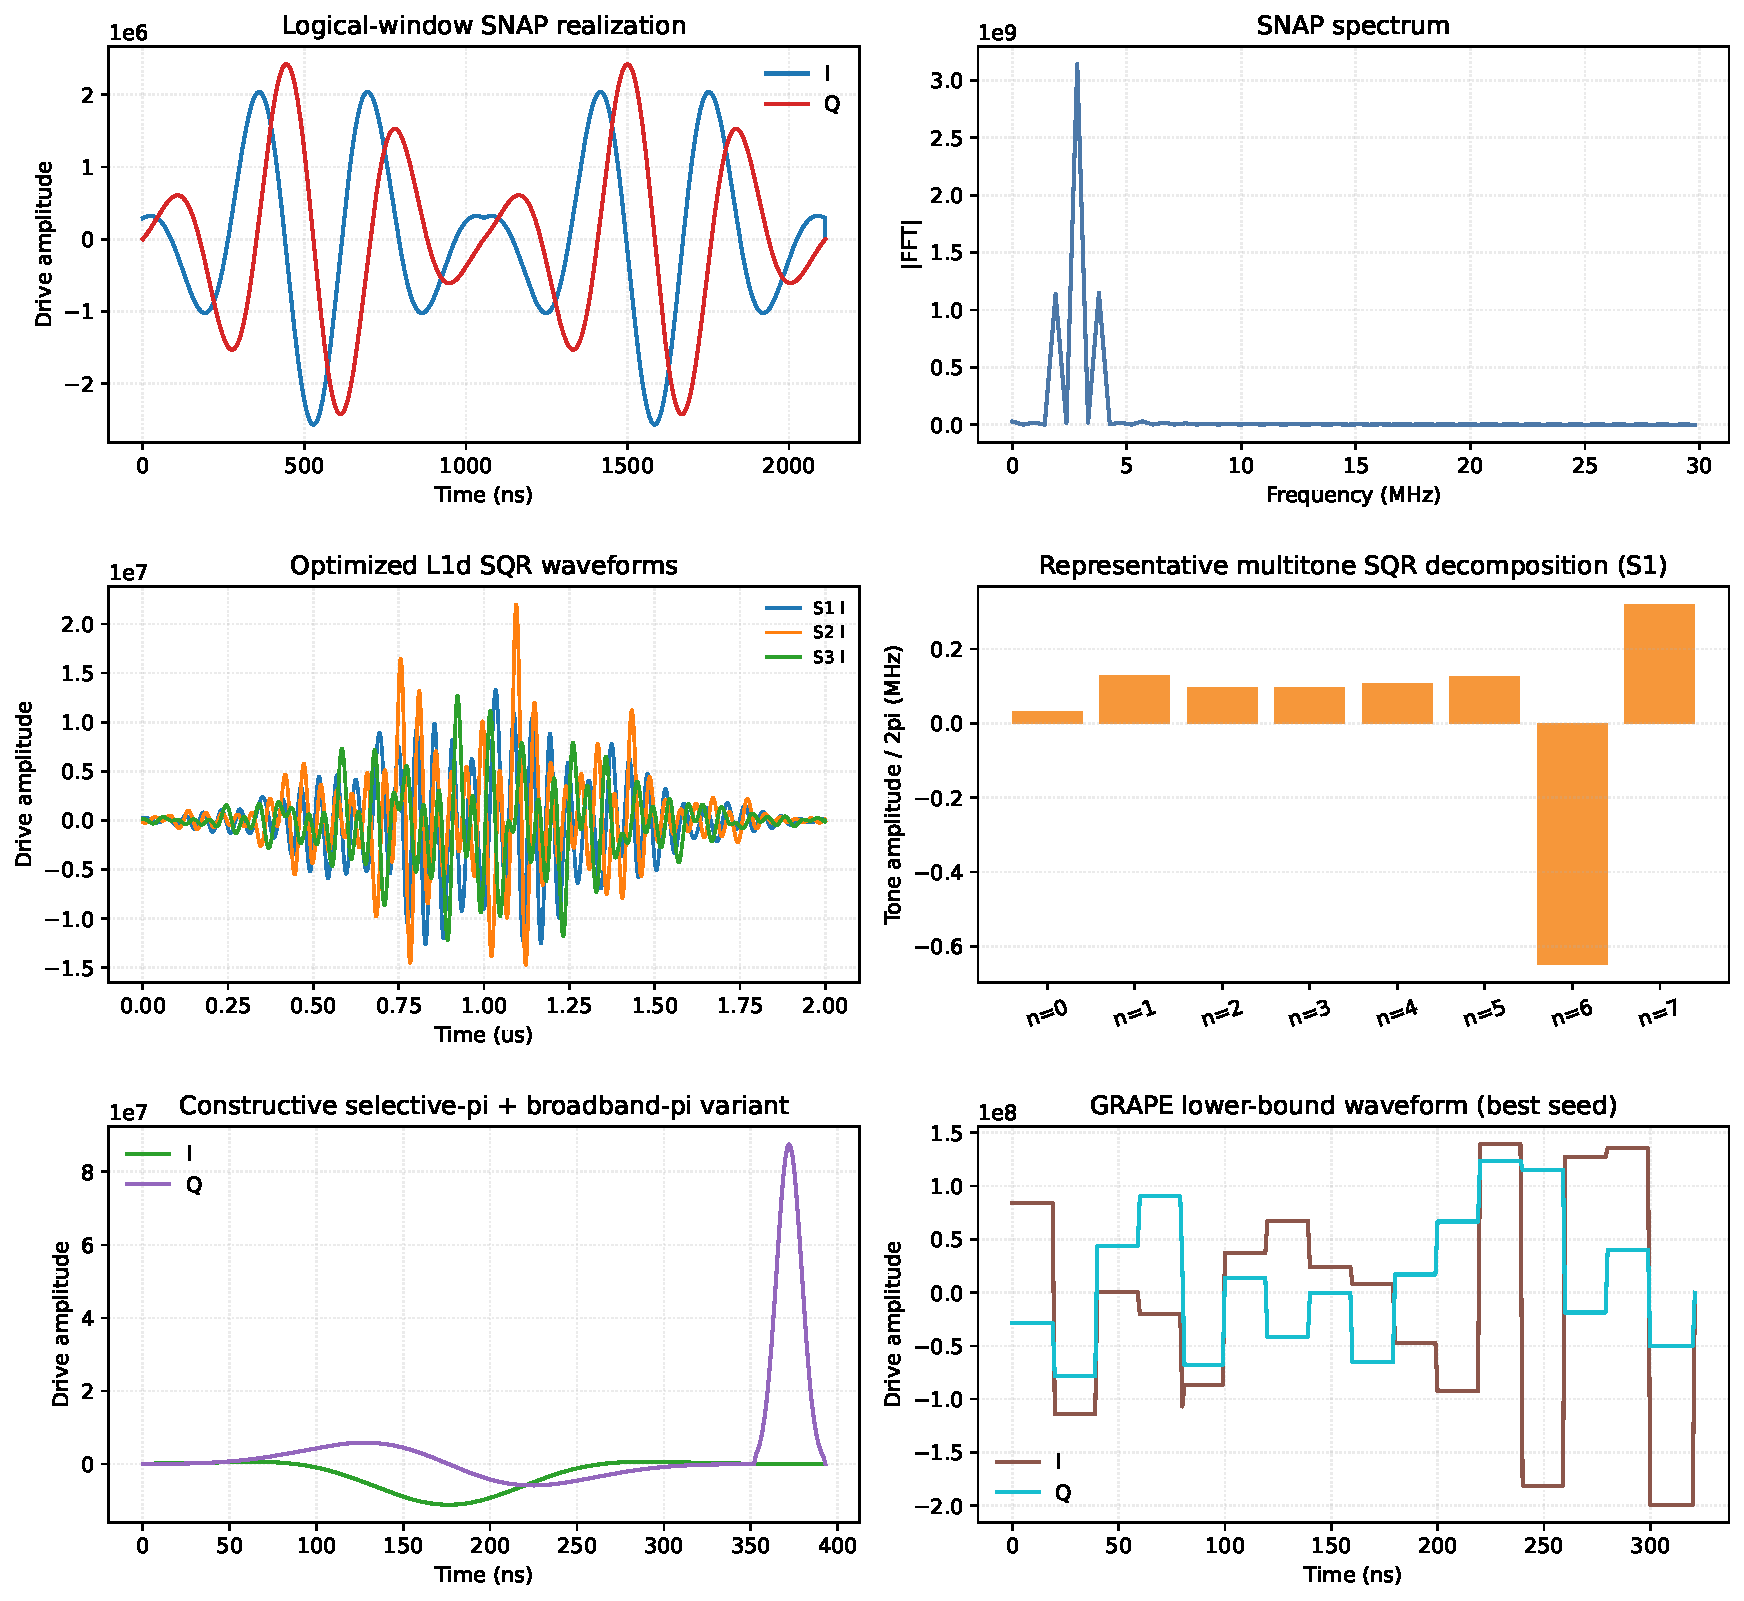
\includegraphics[width=\textwidth]{waveform_realizations.pdf}
\caption{Waveform-level realizations for the pulse-backed part of the follow-up study. Top left: time-domain I/Q envelope of the best logical-window SNAP. Top right: corresponding frequency-domain content. Middle left: the three SQR waveforms from the best $L1d$ sequence after conversion through the \texttt{cqed\_sim} waveform bridge. Middle right: per-Fock multitone amplitudes for the first SQR gate. Bottom left: the constructive shortcut waveform composed of a selective $\pi$ plus a broadband $\pi$. Bottom right: the best GRAPE lower-bound waveform.}
\label{fig:waveforms}
\end{figure}

The mapping from the optimized SQR parameters to physically meaningful pulse content is as follows. The abstract SQR parameters $(\theta_n,\phi_n)$ define a per-Fock selective Bloch rotation. The waveform bridge converts them into a sum of branch-selective tones with frequencies
\begin{equation}
\omega_n \approx n |\chi| + \mathcal{O}(n^2 \chi', n K)
\end{equation}
in the rotating frame, amplitudes proportional to the requested selective rotation strength, and phases inherited from $\phi_n$. For the best $L1d$ sequence, the first SQR gate uses tones from $n=0$ through $7$ with the largest effective amplitudes on the high-$n$ branches, indicating that the optimizer is using strong higher-manifold interference to clean up the logical-block action.

There is an important fairness caveat. The SQR waveforms shown here are pulse-backed. The \texttt{ConditionalPhaseSQR} sequence is not yet pulse-backed because \texttt{cqed\_sim} does not currently export that primitive through the waveform bridge. For that family the report can show exact optimized phase vectors, but not an equivalent calibrated pulse schedule.

\subsection{Optimization Diagnostics and Minimum Checks}

The optimizer evidence is shown in Figures~\ref{fig:diag-structured} and \ref{fig:diag-pulse}. The key conclusions are:
\begin{itemize}
\item multistarts for $A_{\mathrm{local}}$, $D_{\mathrm{ent}}$, $L1c$, $L1d$, and $L2d$ all collapse to essentially identical fidelities, so the reported solutions are not isolated lucky seeds;
\item the extra-displacement test is decisive: $L1c \rightarrow L1d$ improves fidelity from $0.9212$ to $0.9953$, while $L2c \rightarrow L2d$ improves only from $0.8684$ to $0.9135$;
\item the logical SNAP pulse landscape shows a broad high-fidelity region near $\chi T/2\pi \approx 3$ and shape parameter $\approx 0.24$, so the best pulse is not a spiky one-point optimum;
\item the constructive shortcut remains poor across its tested landscape, so its failure is not just a bad initial seed.
\end{itemize}

\begin{figure}[H]
\centering
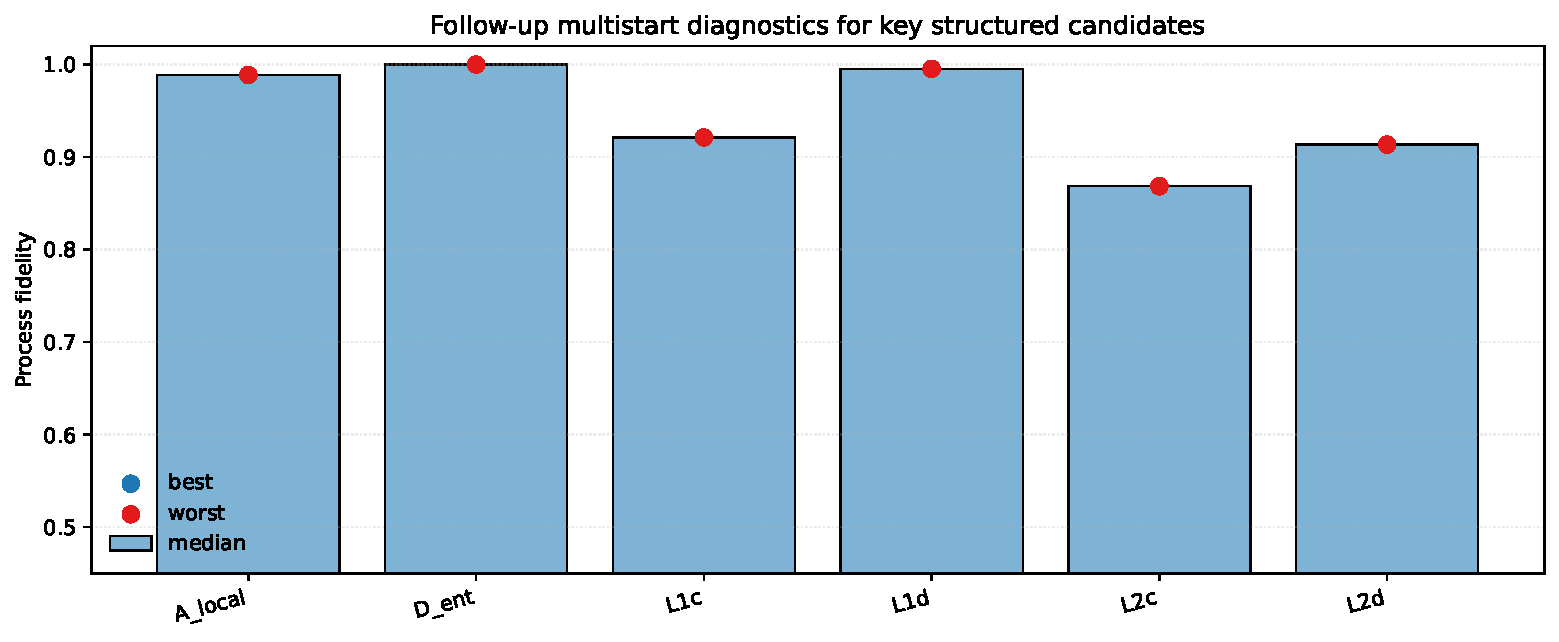
\includegraphics[width=\textwidth]{multistart_statistics.pdf}
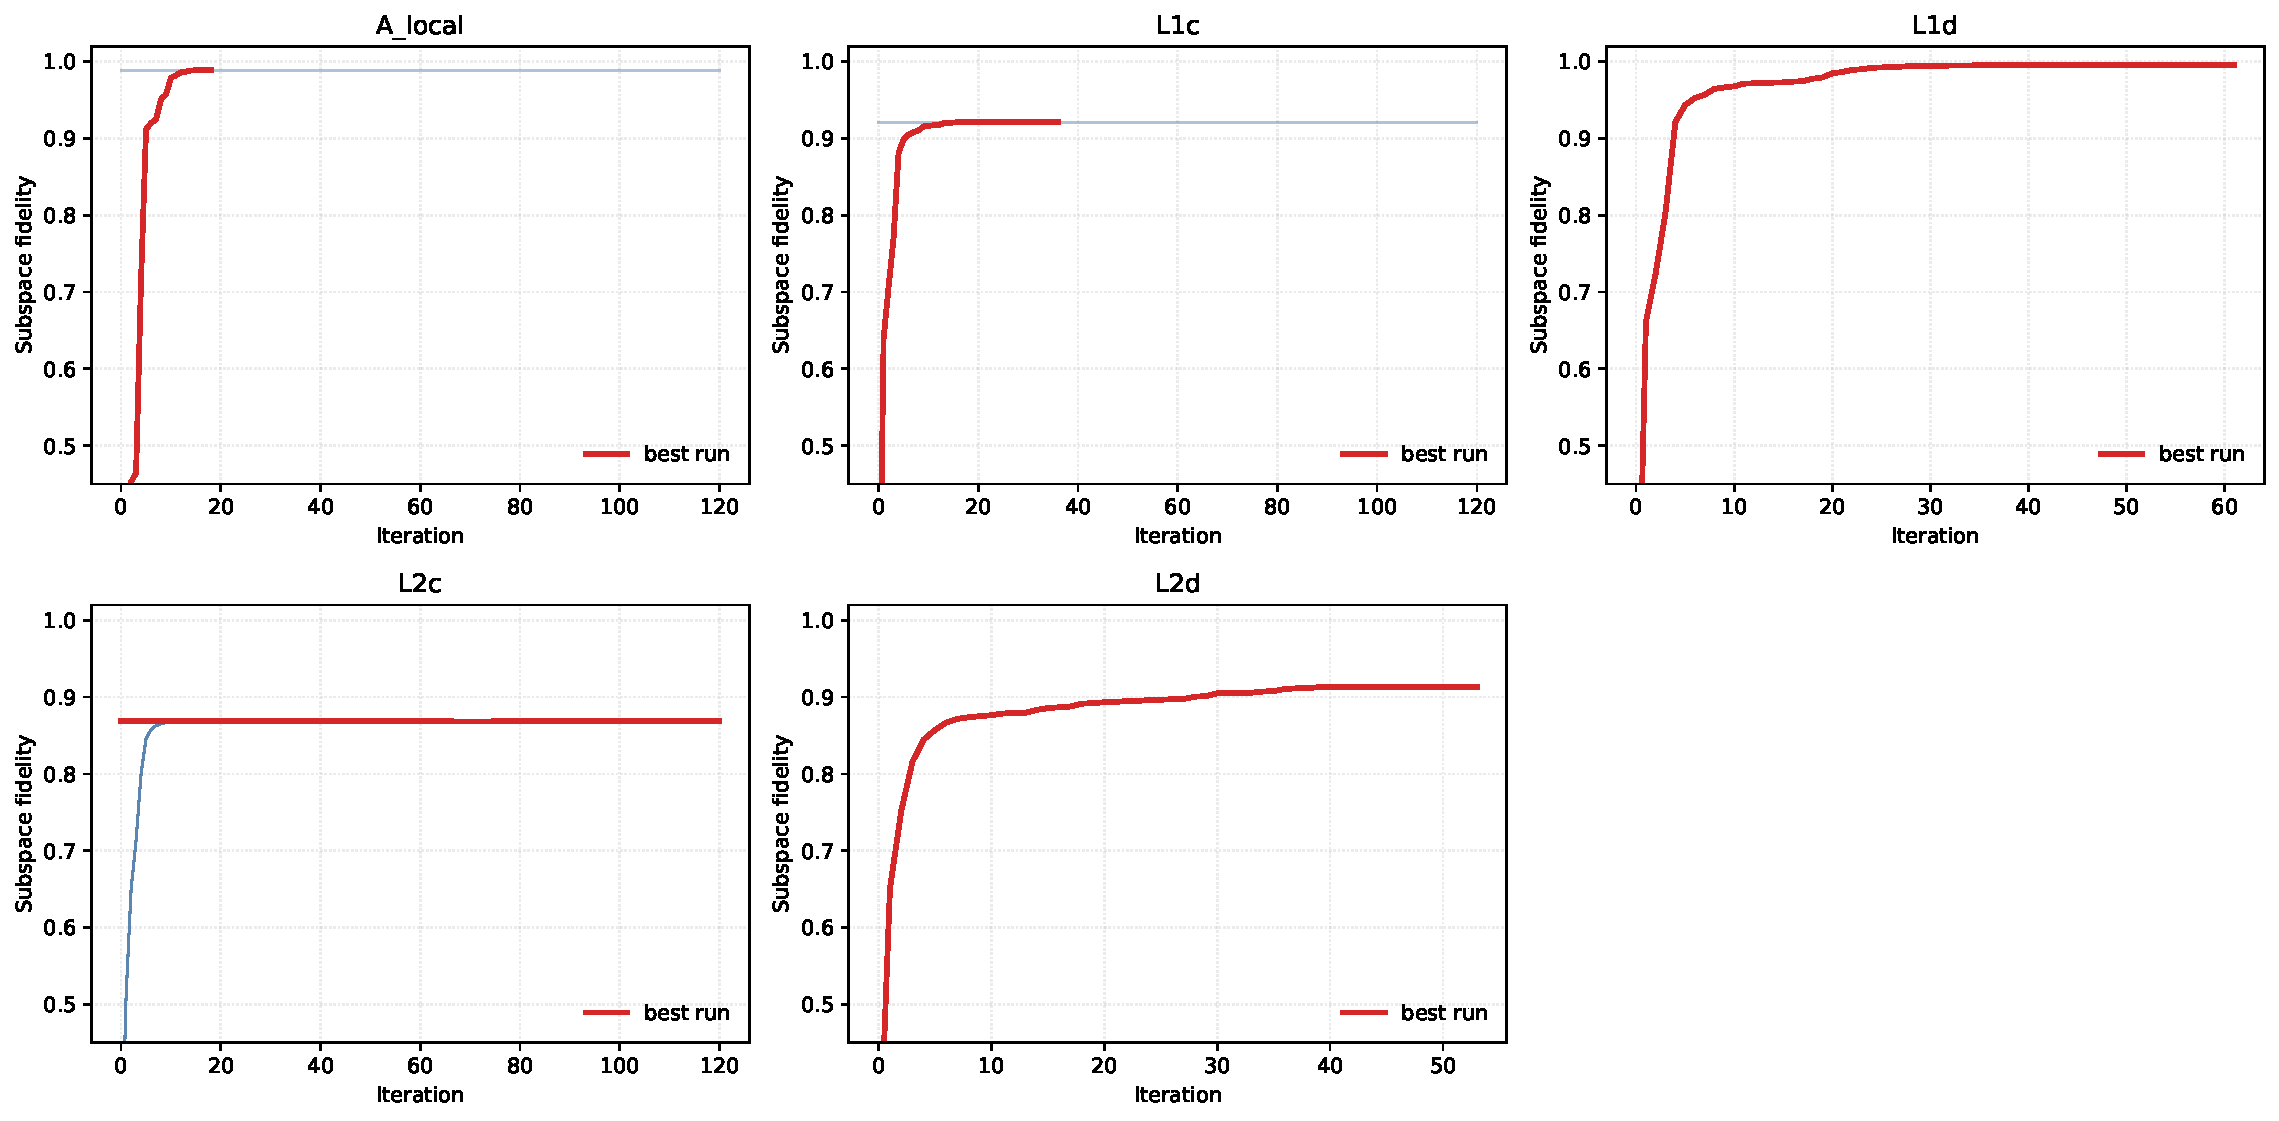
\includegraphics[width=\textwidth]{convergence_histories.pdf}
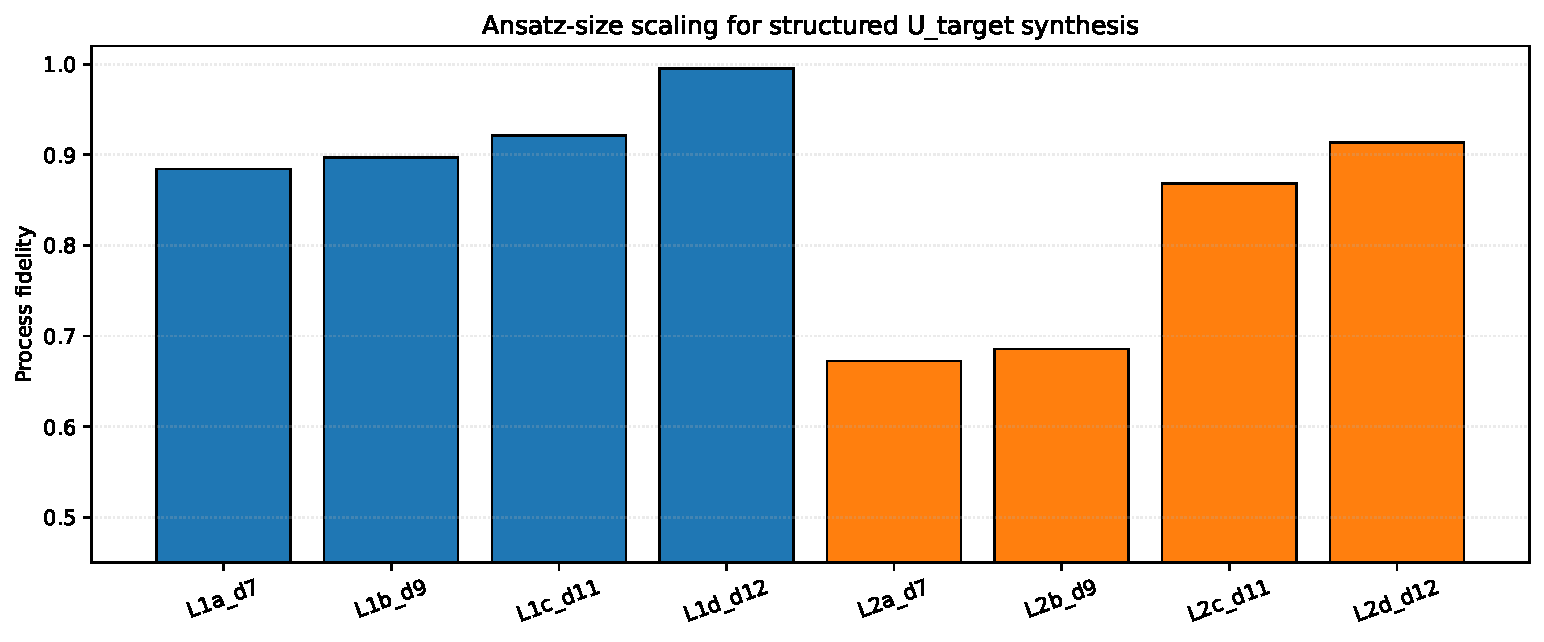
\includegraphics[width=\textwidth]{ansatz_scaling.pdf}
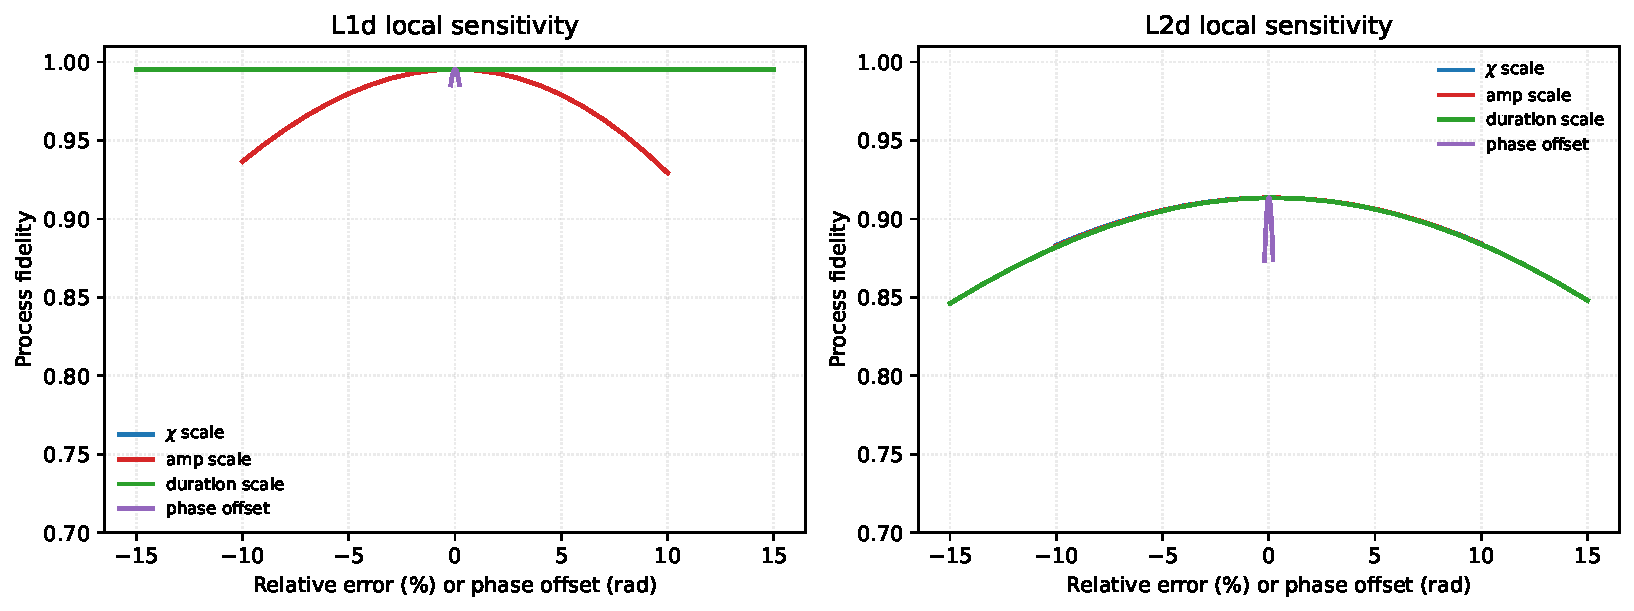
\includegraphics[width=\textwidth]{structured_robustness.pdf}
\caption{Structured optimization diagnostics. From top to bottom: multistart best/median/worst statistics, convergence traces for representative runs, ansatz-size scaling, and local perturbation robustness of the two best structured $U_{\mathrm{target}}$ solutions. The most important feature is the dramatic $L1c \rightarrow L1d$ jump with a single added displacement gate.}
\label{fig:diag-structured}
\end{figure}

\begin{figure}[H]
\centering
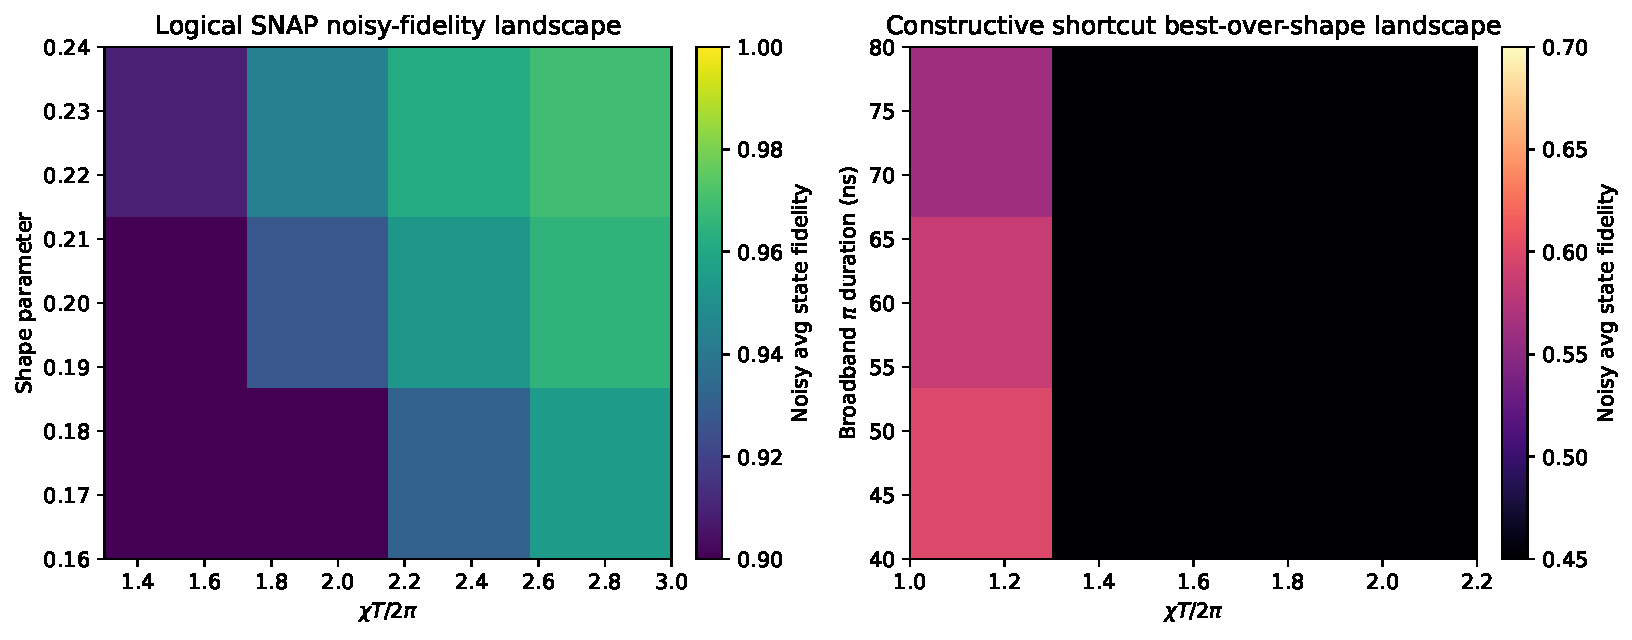
\includegraphics[width=\textwidth]{pulse_landscapes.pdf}
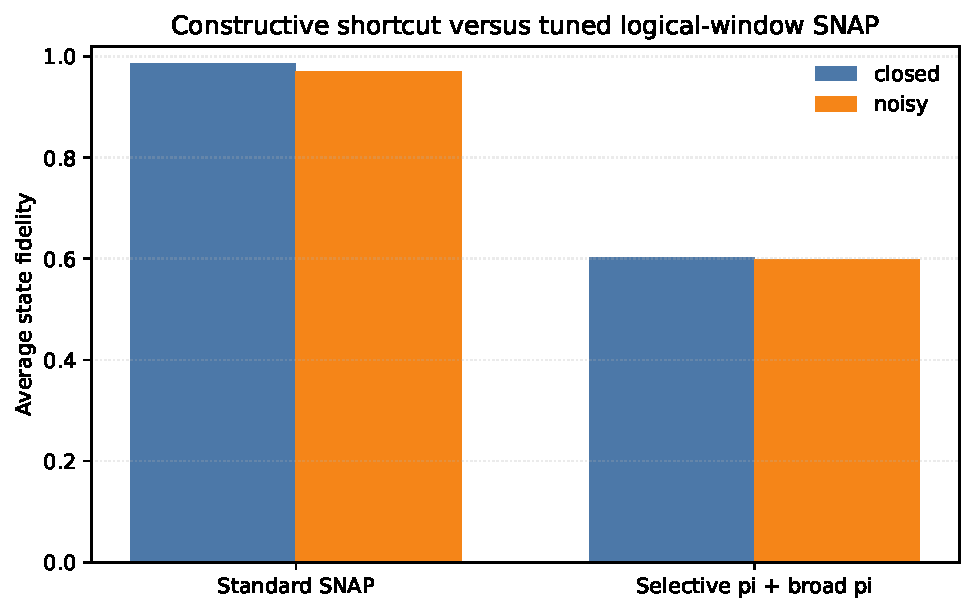
\includegraphics[width=0.72\textwidth]{constructive_variant_comparison.pdf}
\caption{Pulse-level minimum checks. Top: noisy-fidelity landscapes for the logical-window SNAP and for the constructive shortcut. Bottom: best standard SNAP versus best constructive shortcut. The SNAP optimum sits on a usable plateau, while the constructive shortcut remains poor throughout the tested parameter region.}
\label{fig:diag-pulse}
\end{figure}

The local perturbation study refines the deployability picture. $L1d$ is essentially insensitive to $\chi$ scaling and duration scaling over the tested range, while its dominant residual sensitivity is to control amplitude with RMS fidelity drop $0.0085$ over $\pm 5\%$. $L2d$ is more evenly sensitive to $\chi$, amplitude, duration, and phase, each at the few-$10^{-3}$ to few-$10^{-2}$ level. This makes $L1d$ not only more accurate, but easier to calibrate selectively.

\subsection{Constructive ``Selective $\pi$ + Broadband $\pi$'' Variant}

The constructive shortcut was tested numerically because, on paper, it is an attractive logical-subspace idea: use a selective branch-$1$ $\pi$ pulse to imprint the logical selectivity and a fast broadband $\pi$ pulse to complete the effective SNAP-like action without demanding correct behavior on the full oscillator Hilbert space. In practice it fails for this platform and this logical window. The best candidate reaches only
\begin{equation}
F_{\mathrm{avg,closed}} = 0.6020,\qquad
F_{\mathrm{avg,noisy}} = 0.5991.
\end{equation}
The dominant failure mode is not the $|g,1\rangle$ branch, which remains near-correct, but the $|g,0\rangle$ and superposition probes, indicating that the broadband pulse destroys the intended branch discrimination too aggressively. The idea may still have niche value in other encodings or with a more careful echoed construction, but it is not competitive here.

\subsection{Deployable Interpretation}

The revised experiment-facing answer is now more concrete.
\begin{itemize}
\item \textbf{Entangler to deploy first}: native $\chi$-wait plus qubit rotations. It is exact, short, and calibration-light.
\item \textbf{Local logical gate to deploy first}: selective SNAP. The pulse is explicit, the optimum lies on a plateau, and the noisy logical-window fidelity remains near $0.97$.
\item \textbf{Structured universal-control candidate worth deeper implementation work}: $L1d$, the depth-12 $D+R_q+\mathrm{SQR}$ sequence. It is the first structured candidate in this study that simultaneously reaches $\approx 0.995$ logical fidelity and sub-percent average leakage.
\item \textbf{Numerical lower bound only}: GRAPE. It remains useful as a waveform-performance lower bound, but the seed spread and lack of circuit interpretability make it a weaker immediate deployment target than $L1d$ or logical SNAP.
\item \textbf{Not yet hardware-fair}: \texttt{ConditionalPhaseSQR} and the other native effective-interaction primitives without waveform export. Their decomposition numbers are informative, but their calibration burden cannot yet be compared apples-to-apples with pulse-backed controls.
\end{itemize}

\section{Validation}
\label{sec:validation}

\subsection{Sanity Checks}

The native $\chi$-wait entangler still reproduces $\mathrm{CX}(c\!\to\! q)$ to machine precision. The structured follow-up preserved the earlier algebraic result that any ansatz without displacement cannot synthesize the required Fock mixing for $U_{\mathrm{target}}$. The logical-window SNAP follow-up respects the expected selective-pulse hierarchy: longer, more selective pulses improve noisy logical action until diminishing returns set in.

\subsection{Convergence Analysis}

The new structured minima are unusually stable under restart. For $A_{\mathrm{local}}$, $D_{\mathrm{ent}}$, $L1c$, $L1d$, and $L2d$, the best, median, and worst restart fidelities agree to the shown precision. The only visible spread appears in $L2c$, and even there it is in the sixth decimal place. This is strong evidence that the reported optima are stable inside the tested ans\"atze. The logical SNAP optimum also appears on a broad plateau in the waveform-parameter landscape rather than as a needle-like isolated point. Finally, the follow-up tables and figures were regenerated directly from the cached optimization artifacts through the study-local follow-up script, ensuring consistency between the report and the machine-readable outputs.

\subsection{Literature Comparison}

The selective-pulse behavior remains consistent with the SNAP literature~\cite{heeres2015snap,krastanov2015universal,heeres2017logical}: the logical action benefits from longer selectivity windows, while bandwidth-limited shortcuts degrade branch specificity. The ECD-like and conditional-displacement underperformance in the strict Fock encoding remains consistent with the fact that those methods are more naturally matched to displacement-oriented encodings~\cite{eickbusch2022ecd,diringer2024cnod}. The persistent dominance of the native $\chi$-wait entangler aligns with the broader lesson from native-interaction work~\cite{yang2024nativecubic}: when the Hamiltonian already supplies the correct nonlinearity, elaborate synthesis may lose to the direct route.

\section{Discussion}
\label{sec:discussion}

The main scientific change introduced by this follow-up is that the previous $U_{\mathrm{target}}$ synthesis bottleneck was not a fundamental leakage ceiling of the structured SQR family. It was an ansatz ceiling. Adding a single extra displacement gate changes the best structured solution from a clearly imperfect $0.92$-fidelity circuit into a high-quality $0.995$-fidelity circuit with very low leakage. That is exactly the kind of result that justifies a follow-up study: the optimizer was not merely polishing the old answer, it found a qualitatively better regime.

This does not mean the structured SQR family has become the universal answer to every control problem. The sequence is still long at \SI{7.3}{\micro s}, and the high-$n$ tone content in the first SQR gate indicates nontrivial calibration burden. What changed is that the family is now credible as a structured, interpretable universal-control candidate rather than only an existence proof with noticeable logical error.

The native-versus-selective split also remains experimentally important. If the goal is a single entangling primitive, the native $\chi$-wait route is still the clear winner. If the goal is a selective local oscillator phase gate with an explicit waveform, logical SNAP is cleaner than the more elaborate structured universal sequence. This argues for a staged experimental program:
\begin{itemize}
\item deploy native $\chi$-wait entanglement first;
\item keep selective SNAP as the default local logical primitive;
\item treat $L1d$ as the main structured-circuit candidate for a deeper waveform-compilation effort;
\item use GRAPE as a lower-bound reference, not the first production path.
\end{itemize}

The remaining fairness limitation is important and should not be blurred away. The report now contains pulse-backed logical SNAP and pulse-backed SQR waveforms, but the CP family is still only represented at the ideal decomposition level. Until waveform export exists for \texttt{ConditionalPhaseSQR}, any conclusion that one structured family is harder or easier to deploy than the other must remain provisional.

\section{Conclusion}

The follow-up study changed the hybrid-universal-control story in a substantive way.
\begin{itemize}
\item The native $\chi$-wait entangler remains the best deployable entangling primitive: $F_{\mathrm{proc}} = 0.9999999$ in \SI{256}{ns} with zero leakage.
\item The best local logical gate remains selective SNAP-based control. The tuned logical-window SNAP reaches closed and noisy logical average state fidelities of $0.9857$ and $0.9694$, respectively.
\item The best structured universal-control candidate is no longer the old depth-11 SQR ansatz. The new depth-12 $L1d$ circuit reaches $F_{\mathrm{proc}} = 0.9953$ with $L_{\mathrm{avg}} = 0.0065$.
\item The CP-based structured family improves with an added displacement gate but remains substantially worse at $F_{\mathrm{proc}} = 0.9135$.
\item The constructive ``selective $\pi$ plus broadband $\pi$'' shortcut is not viable in the present logical window, plateauing near $0.60$ fidelity.
\item Multistarts, convergence histories, ansatz scaling, waveform landscapes, and local perturbation studies all support the conclusion that the reported winners are meaningful optima within their tested ans\"atze rather than obviously poor local minima.
\end{itemize}

For the next hardware-facing step, the most actionable path is a mixed strategy: native $\chi$-wait for entanglement, selective SNAP for immediate local logical control, and the new $L1d$ structured circuit as the main target for a future pulse-compilation and noisy-replay campaign.

\section{Limitations and Future Work}
\label{sec:limitations}

\subsection{Known Limitations}
\begin{itemize}
\item \textbf{Encoding scope}: all results remain specific to the strict Fock $\{|0\rangle, |1\rangle\}$ encoding. The ranking may change for cat, binomial, or larger Fock encodings.
\item \textbf{Waveform-bridge coverage}: \texttt{SNAP} and \texttt{SQR} can now be represented physically in this study, but \texttt{ConditionalPhaseSQR}, \texttt{ConditionalDisplacement}, and native exchange primitives still lack full waveform export in the present workflow. Their implementation readiness is therefore lower than their decomposition-level numbers suggest.
\item \textbf{Two-level synthesis loop}: the structured unitary-synthesis optimization still uses $n_\mathrm{tr}=2$. Pulse-backed replay uses $n_\mathrm{tr}=3$, but the structured decomposition ranking still omits direct $|f\rangle$ leakage during optimization.
\item \textbf{Structured-sequence duration}: the best $L1d$ circuit is accurate but long. At \SI{7.3}{\micro s}, coherence will matter in any real deployment.
\item \textbf{Ansatz ceiling not globally closed}: the follow-up shows that the old depth-11 plateau was not final, but it does not prove that depth-12 is globally optimal among all short structured circuits.
\item \textbf{Single device point}: only one representative cQED parameter set was studied. Different $\chi/\alpha$ ratios or cavity Kerr values could change the balance between selectivity and speed.
\end{itemize}

\subsection{Suggested Improvements}
\begin{itemize}
\item \textbf{[P1 | HIGH]} Add waveform export for \texttt{ConditionalPhaseSQR} and the native effective-interaction primitives, then repeat the follow-up with pulse-backed fairness across all leading families.
\item \textbf{[P1 | MEDIUM]} Replay $L1d$ with explicit noise and $n_\mathrm{tr}=3$ inside the optimization loop. The present report shows coherent robustness, but not a full noisy synthesis objective.
\item \textbf{[P2 | MEDIUM]} Extend the depth-plus-one search to further structured variants, including SNAP-assisted circuits, to test whether $L1d$ is near-minimal or simply the first large jump.
\item \textbf{[P2 | MEDIUM]} Repeat the selective-pulse follow-up for cat-like and binomial encodings. The constructive shortcut may fail in the Fock block yet still be useful elsewhere.
\item \textbf{[P2 | LOW]} Use the extracted $L1d$ tone table as a starting point for calibration-aware pulse compression, for example by pruning weak tones or constraining branch phases.
\item \textbf{[P3 | MEDIUM]} Warm-start GRAPE from the structured $L1d$ waveform realization to test whether the interpretable circuit already sits near the pulse-level lower bound.
\end{itemize}

\subsection{Open Questions}
\begin{itemize}
\item Is the extra displacement in $L1d$ the minimal structural ingredient that resolves the previous $U_{\mathrm{target}}$ bottleneck, or would a shorter SNAP-assisted circuit achieve similar quality?
\item Can the high-$n$ tones in the optimized SQR gates be compressed into a more calibration-friendly selective pulse without losing the logical fidelity gain?
\item Does the native exchange family become comparatively stronger once the logical encoding is no longer the strict $\{|0\rangle,|1\rangle\}$ Fock block?
\item How much of the remaining gap between $L1d$ and the ideal limit is coherent controllability, and how much is simply the cost of keeping the circuit interpretable?
\end{itemize}

\bibliographystyle{unsrtnat}
\bibliography{references}

\end{document}
